\subsection{The action of $\PSL{\Z}$ on $\EC$}

In Theorem~\ref{thm_SL2FunDomAlg} we have seen an algorithm which naturally gives rise to a set $\hat{\mathcal{R}} \subseteq \C^2$ which can easily be restricted to a subset $\hat{\FunDom} \subseteq \hat{\mathcal{R}}$ being a fundamental region for the action of $\SL{\Z}$ on $\hat{\mathcal{S}}$. We can exploit this fact in search of a fundamental region for the action on of the (inhomogeneous) modular group $\PSL{\Z}$ on $\EC$. For this purpose we project $\C^2$ onto $\EC$ using the map $\pi : \C^2 \to \EC$,
\begin{equation}
\pi : \cvec{u}{v} \mapsto \frac{u}{v}.
\end{equation}
Let us first consider image of $\hat{\mathcal{S}}$ under $\pi$. If $({}^u_v) \in \hat{\mathcal{S}}$, then by definition $u$ and $v$ are linear independent over $\R$ or linear dependent over $\Q$. In the first case we have $\frac{u}{v} \in \C \setminus \R$ and in the second case $\frac{u}{v} \in \Q \cup \{\infty\}$. This means $\frac{u}{v}$ may be everything but irrational. Denoting set of irrational numbers by $\Irrat = \R \setminus \Q$, we thus have
\begin{equation*}
\pi(\hat{\mathcal{S}}) = \EC \setminus \Irrat.
\end{equation*}
Projection of the set $\hat{\mathcal{R}} \subseteq \C^2$ leads to the region $\mathcal{R} \subseteq \EC$ (see also Figure~\ref{fig_PSL2MinRegion}),
\begin{equation}
\label{eqn_PSL2MinRegion}
\mathcal{R} := \pi\left(\hat{\mathcal{R}}\right) = 
\setdefsz{\Big}{\frac{u}{v} \in \EC}{\abs{u\conj{v} + \conj{u}v} < \min\{\abs{u}^2, \abs{v}^2\}}.
\end{equation}
\begin{figure}
\centering
\includegraphics[width=0.8\textwidth]{figures/minimal-region}
\caption{The region $\mathcal{R} \subseteq \EC$ of numbers $z = u/v \in \EC$ with $\abs{u\conj{v} + \conj{u}v} < \min\{\abs{u}^2,\abs{v}^2\}$. It is obtained by taking the strip $\setdefsz{\big}{z \in \C}{\abs{\Re{z}} < \reci{2}}$  and cutting out two closed disks of unit radius centered about the real points $\pm 1$. The arising vertices are labeled. As usual, $T$ is the transformation $z \mapsto -\reci{z}$ and $\rho = \exp(2 \pi \ii / 3)$ is a third root of unity.}
\label{fig_PSL2MinRegion}
\end{figure}
It follows that $\mathcal{R}$ contains a fundamental region for the action of $\PSL{\Z}$ on $\EC \setminus \Irrat$. As in the homogeneous case, we see from Theorem~\ref{thm_SL2FunDomGlobMin} that equivalence of points within $\mathcal{R}$ can be established only by powers of the transformation $T \in \PSL{\Z}$. Since $T^2 = 1$, in order to obtain a fundamental region we now need to choose for each $z \in \mathcal{R}$ just exactly one of the equivalent points $z$ and $Tz$. This can for example be done such that $\abs{z} > 1$.

\index{Extended upper halfplane}
Note that for understanding the group action of $\PSL{\Z}$ on $\EC \setminus \Irrat$ it is sufficient to look at either the upper or lower halfplane of $\C$, since the group action one halfplane can be easily understood from the group action on the other halfplane, as we trivially have $Az = \conj{A\conj{z}}$. Let us therefore denote by $\mathcal{H}$ the upper halfplane and by $\EU$ the \emph{extended upper halfplane}:
\begin{eqnarray}
\label{eqn_UpperHalfplane}\mathcal{H} &:=& \setdefsz{\big}{z \in \C}{\Im{z} > 0} \\
\label{eqn_ExtUpperHalfplane}
\EU &:=& \mathcal{H} \cup \Q \cup \{\infty\}.
\end{eqnarray}
Clearly $\EU$ is invariant under $\PSL{\Z}$, \ie $\PSL{\Z} \EU = \EU$ and we can also consider $\PSL{\Z}$ acting on $\EU$.

\begin{theorem}
\label{thm_PSL2FunDom}
Let $\mathcal{H}$ and $\EU$ be defined as above. The set
\begin{equation}
\tilde{\FunDom} := \setdefsz{\bigg}{z \in \C}{\abs{\Re{z}} < \reci{2} \text{ and } \abs{z} > 1}
\end{equation}
is a fundamental region for the action of $\PSL{\Z}$ on $\EC \setminus \Irrat$. The part of $\tilde{\FunDom}$ lying in the upper halfplane $\mathcal{H}$, \ie the set
\begin{equation}
\label{eqn_PSL2FunDom}
\FunDom := \tilde{\FunDom} \cap \mathcal{H}
\end{equation}
is a fundamental region for the action of $\PSL{\Z}$ on $\EU$.
\end{theorem}
\begin{proof}
The second statement that $\FunDom = \tilde{\FunDom} \cap \mathcal{H}$ is fundamental region for $\PSL{\Z}$ acting on $\EU$ is a simple consequence of the first statement. For proving that $\tilde{\FunDom}$ is fundamental,  observe that $\tilde{\FunDom}$ is exactly the set
\begin{equation*}
\tilde{\FunDom} = \mathcal{R} \cap \setdef{z \in \C}{\abs{z} > 1},
\end{equation*}
with $\mathcal{R}$ as in (\ref{eqn_PSL2MinRegion}) -- compare also Figure~\ref{fig_PSL2MinRegion}. Obviously $\tilde{\FunDom}$ is a nonempty open subset of $\mathcal{R}$, which is why two distinct points of $\tilde{\FunDom}$ can be equivalent only by the transformation $T$. However, since $\abs{z} > 1$ implies $\abs{Tz} = \abs{-1/z} < 1$, this is impossible. Therefore $\tilde{\FunDom}$ contains no equivalent distinct points.

It remains to show that every $z = \frac{u}{v} \in \mathcal{S}$ is equivalent to a point of the topological closure $\topcl{\tilde{\FunDom}}$ of $\tilde{\FunDom}$. For this purpose apply the algorithm of Theorem~\ref{thm_SL2FunDomAlg} to the vector $({}^u_v) \in \hat{\mathcal{S}}$ in order to obtain a transformation $B \in \PSL{\Z}$ which maps $z$ to a point of $\topcl{\mathcal{R}}$. It then follows that at least one of the points $Bz$ or $TBz$ lies in $\topcl{\tilde{\FunDom}}$.
\end{proof}

We now wish to obtain a \emph{fundamental set} for the action of $\PSL{\Z}$ on $\EU$. For this purpose we need to consider the boundary of $\FunDom$ and to investigate equivalent boundary points and their associated transformations. It turns out that we can define a fundamental set for the action of $\PSL{Z}$ on $\EU$ the following way:

\begin{theorem}[The fundamental set $\FunSet$]
\label{thm_PSL2FunSet}
Denote by $\FunDom$ the fundamental region from (\ref{eqn_PSL2FunDom}). The boundary of $\FunDom$ shall be segmented into the four ``boundary arcs'',
\begin{eqnarray*}
a &:=& \setdefsz{\bigg}{-\reci{2} + y \ii}{y \ge \frac{\sqrt{3}}{2}} \cup \{\infty\},\\
b &:=& \setdefsz{\bigg}{+\reci{2} + y \ii}{y \ge \frac{\sqrt{3}}{2}} \cup \{\infty\},\\
c &:=& \setdefsz{\Big}{\ii \epo{+\ii \phi}}{0 \le \phi \le \frac{\pi}{6}},\\
d &:=& \setdefsz{\Big}{\ii \epo{-\ii \phi}}{0 \le \phi \le \frac{\pi}{6}}.
\end{eqnarray*}
These boundary arcs are mapped onto each other by $Ua = b$ and $Tc = d$. The set
\begin{equation}
\label{eqn_PSL2FunSet}
\FunSet := \FunDom \cup a \cup c
\end{equation}
is a fundamental set for the action of $\PSL{\Z}$ on the extended upper halfplane $\EU$.
\end{theorem}
\begin{proof}
It follows from Theorem~\ref{thm_SL2FunDomGlobMin} that equivalence of boundary points of $\FunDom$ can only be established by transformations $A \in \PSL{Z}$ with $n(A) \le 3$. The full list of candidate transformations therefore comprises of 9 transformations: $T$, $U$, $TU$, $UT$, $TUT$ and the respective inverse transformations (note that $T$ is self-inverse). After looking at these transformations individually, it turns out that in fact only $T$ and $U$ (and $\inv{U}$) map boundary points to boundary points. Indeed $Ua = b$ and $Tc = d$ can readily be seen.
\end{proof}

\begin{remark}
\label{rem_PSL2FunDomGenDisks}
\begin{figure}
\centering
\includegraphics[width=0.8\textwidth]{figures/fundom}
\caption{The fundamental domain $\FunDom$ for the action of the modular group $\PSL{\Z}$ on the extended upper halfplane $\EU$. It is bounded by ``generalized arcs'' $a$, $b$, $c$ and $d$ which correspond to the generalized disks $\mathbb{A}$, $\mathbb{B}$ and the unit disk $\mathbb{D}$. There is a unique disk $\mathcal{I}$ which is tangent $\mathbb{A}$, $\mathbb{B}$ and $\mathbb{D}$.}
\label{fig_PSL2FunDom}
\end{figure}
In Figure~\ref{fig_PSL2FunDom}, we see that the fundamental region $\FunDom$ can also be described in terms of generalized disks (see Definition~\ref{dfn_GenDisk}): With the terminology of Theorem~\ref{thm_PSL2FunSet}, the boundary arcs $a$ and $b$ are indeed ``generalized arcs'' of the closed generalized disks
\begin{equation*}
\mathbb{A} := \mat{0}{1}{1}{1} \quad \text{and} \quad \mathbb{B} := \mat{\phantom{+}0}{-1}{-1}{\phantom{+}1}
\end{equation*}
respectively. The boundary arcs $c$ and $d$ are part of the boundary of the closed unit disk
\begin{equation*}
\mathbb{D} := \mat{1}{\phantom{+}0}{0}{-1}.
\end{equation*}
We see that the fundamental region $\FunDom$ can be characterized as set complement of the union of these three closed g-disks:
\begin{equation*}
\FunDom = \EU \setminus \left(\mathbb{A} \cup \mathbb{B} \cup \mathbb{D}\right).
\end{equation*}
Moreover there exists a unique (open) disk $\mathcal{I} \subseteq \FunDom$, which is tangent to $\mathbb{A}$, $\mathbb{B}$ and $\mathbb{D}$ which we may the \emph{indisk} $\mathcal{I}$ of $\FunDom$.
\end{remark}

The fact that $\FunSet$ is a fundamental set for the action of $\PSL{\Z}$ on $\EU$ can be reformulated as follows: For every point $z \in \EU$ there exists a unique transformation $A \in \PSL{\Z}$ such that $z \in A \FunSet$. In order to determine this transformation, we can adopt the algorithm of Theorem~\ref{thm_SL2FunDomAlg}:

\begin{theorem}[The fundamental set algorithm]
Let $z \in \EU$ be a point of the extended upper halfplane and the fundamental set $\FunSet$ be defined as above. The unique transformation $A$ satisfying $z \in A \FunSet$ can be found by performing the following steps:
\begin{enumerate}
\item Set $j := -1$ and $B_0 := 1$.
\item \label{itm_PSL2FunSetAlgLoop}
Increment $j$ by one and set $z_j := B_j z$. If $z_j \in \FunSet$, then goto step \ref{itm_PSL2FunSetAlgDone}.
\item \label{itm_PSL2FunSetAlgEjDef}
Set $e_j := \floor{\Re{z_j} + \reci{2}}$. 
\item \label{itm_PSL2FunSetAlgNext}
If $z_j - e_j \in \FunSet$, set $B_{j+1} := U^{-e_j}B_j$ -- else set $B_{j+1} := TU^{-e_j}B_j$.
\item Continue with step \ref{itm_PSL2FunSetAlgLoop}.
\item \label{itm_PSL2FunSetAlgDone} 
The desired matrix $A$ is given by $A = \inv{B_j}$.
\end{enumerate}
\end{theorem}
\begin{proof}
Note that the above is essentially a reformulation of the algorithm of Theorem~\ref{thm_SL2FunDomAlg} with the following modifications:
\begin{enumerate}[\quad (a)]
\item The algorithm is reformulated for the inhomogeneous case. The numbers $z_j$ from above and the vectors $x_j$ from the proof of Theorem~\ref{thm_SL2FunDomAlg} correspond by $z_j = \pi(x_j)$.
\item \label{itm_PSL2FunDomAlgModNint}
Instead of using the $\nint{}$ function, we use the above definition  for determining the coefficients $e_j$ -- see step \ref{itm_PSL2FunSetAlgEjDef}. This is to ensure that $z_j - e_j \in [-\reci{2}, \reci{2})$ -- otherwise we would have problems with the termination of the algorithm for the case when some $z_j$ lies on the boundary arc $b$ (as defined in Theorem~\ref{thm_PSL2FunSet}).
\item Theorem~\ref{thm_SL2FunDomAlg} yields a final vector $x_n$ such that $w := \pi(x_n) \in \topcl{\mathcal{R}}$, where $\mathcal{R}$ is defined as in (\ref{eqn_SL2MinRegionDef}). In order to obtain a point in $\FunSet \subseteq \topcl{\mathcal{R}}$, we need to apply to $w$ possibly $T$ and -- if this point lies on the boundary arc $b$ -- possibly $U^{-1}$. We take this into account by explicitly checking whether the application of $T$ in the last iteration of the algorithm is necessary or not (see step \ref{itm_PSL2FunSetAlgNext}) and by the modification discussed in (\ref{itm_PSL2FunDomAlgModNint}).\qedhere
\end{enumerate}
\end{proof}

%Now that we have found a fundamental region and fundamental set, we will investigate how they are mapped by modular transformations. Here it is beneficial to use an alternative description of the fundamental region $\FunDom$ in terms of generalized disks (see Definition~{\ref{dfn_GenDisk}}).  

\begin{figure}
\centering
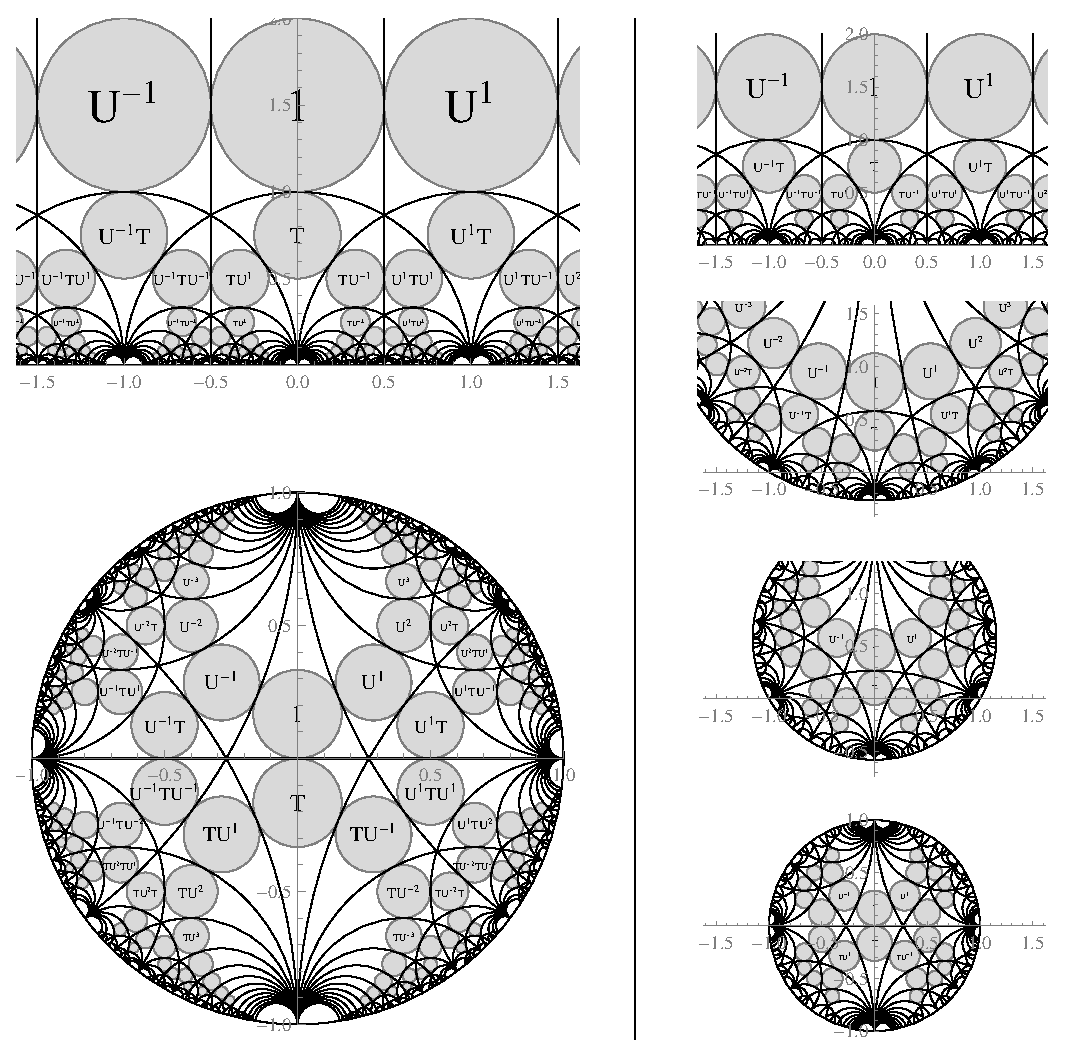
\includegraphics[width=\textwidth]{figures/modular-tiling-1}
\caption{The tessellation of the upper halfplane.}
\label{fig_ModularTiling}
\end{figure}
